% Options for packages loaded elsewhere
\PassOptionsToPackage{unicode}{hyperref}
\PassOptionsToPackage{hyphens}{url}
\PassOptionsToPackage{dvipsnames,svgnames,x11names}{xcolor}
\documentclass[
  11pt,
]{article}
\usepackage{xcolor}
\usepackage[margin=1in]{geometry}
\usepackage{amsmath,amssymb}
\setcounter{secnumdepth}{5}
\usepackage{iftex}
\ifPDFTeX
  \usepackage[T1]{fontenc}
  \usepackage[utf8]{inputenc}
  \usepackage{textcomp} % provide euro and other symbols
\else % if luatex or xetex
  \usepackage{unicode-math} % this also loads fontspec
  \defaultfontfeatures{Scale=MatchLowercase}
  \defaultfontfeatures[\rmfamily]{Ligatures=TeX,Scale=1}
\fi
\usepackage{lmodern}
\ifPDFTeX\else
  % xetex/luatex font selection
\fi
% Use upquote if available, for straight quotes in verbatim environments
\IfFileExists{upquote.sty}{\usepackage{upquote}}{}
\IfFileExists{microtype.sty}{% use microtype if available
  \usepackage[]{microtype}
  \UseMicrotypeSet[protrusion]{basicmath} % disable protrusion for tt fonts
}{}
\makeatletter
\@ifundefined{KOMAClassName}{% if non-KOMA class
  \IfFileExists{parskip.sty}{%
    \usepackage{parskip}
  }{% else
    \setlength{\parindent}{0pt}
    \setlength{\parskip}{6pt plus 2pt minus 1pt}}
}{% if KOMA class
  \KOMAoptions{parskip=half}}
\makeatother
\usepackage{longtable,booktabs,array}
\usepackage{calc} % for calculating minipage widths
% Correct order of tables after \paragraph or \subparagraph
\usepackage{etoolbox}
\makeatletter
\patchcmd\longtable{\par}{\if@noskipsec\mbox{}\fi\par}{}{}
\makeatother
% Allow footnotes in longtable head/foot
\IfFileExists{footnotehyper.sty}{\usepackage{footnotehyper}}{\usepackage{footnote}}
\makesavenoteenv{longtable}
\usepackage{graphicx}
\makeatletter
\newsavebox\pandoc@box
\newcommand*\pandocbounded[1]{% scales image to fit in text height/width
  \sbox\pandoc@box{#1}%
  \Gscale@div\@tempa{\textheight}{\dimexpr\ht\pandoc@box+\dp\pandoc@box\relax}%
  \Gscale@div\@tempb{\linewidth}{\wd\pandoc@box}%
  \ifdim\@tempb\p@<\@tempa\p@\let\@tempa\@tempb\fi% select the smaller of both
  \ifdim\@tempa\p@<\p@\scalebox{\@tempa}{\usebox\pandoc@box}%
  \else\usebox{\pandoc@box}%
  \fi%
}
% Set default figure placement to htbp
\def\fps@figure{htbp}
\makeatother
% definitions for citeproc citations
\NewDocumentCommand\citeproctext{}{}
\NewDocumentCommand\citeproc{mm}{%
  \begingroup\def\citeproctext{#2}\cite{#1}\endgroup}
\makeatletter
 % allow citations to break across lines
 \let\@cite@ofmt\@firstofone
 % avoid brackets around text for \cite:
 \def\@biblabel#1{}
 \def\@cite#1#2{{#1\if@tempswa , #2\fi}}
\makeatother
\newlength{\cslhangindent}
\setlength{\cslhangindent}{1.5em}
\newlength{\csllabelwidth}
\setlength{\csllabelwidth}{3em}
\newenvironment{CSLReferences}[2] % #1 hanging-indent, #2 entry-spacing
 {\begin{list}{}{%
  \setlength{\itemindent}{0pt}
  \setlength{\leftmargin}{0pt}
  \setlength{\parsep}{0pt}
  % turn on hanging indent if param 1 is 1
  \ifodd #1
   \setlength{\leftmargin}{\cslhangindent}
   \setlength{\itemindent}{-1\cslhangindent}
  \fi
  % set entry spacing
  \setlength{\itemsep}{#2\baselineskip}}}
 {\end{list}}
\usepackage{calc}
\newcommand{\CSLBlock}[1]{\hfill\break\parbox[t]{\linewidth}{\strut\ignorespaces#1\strut}}
\newcommand{\CSLLeftMargin}[1]{\parbox[t]{\csllabelwidth}{\strut#1\strut}}
\newcommand{\CSLRightInline}[1]{\parbox[t]{\linewidth - \csllabelwidth}{\strut#1\strut}}
\newcommand{\CSLIndent}[1]{\hspace{\cslhangindent}#1}
\setlength{\emergencystretch}{3em} % prevent overfull lines
\providecommand{\tightlist}{%
  \setlength{\itemsep}{0pt}\setlength{\parskip}{0pt}}
\usepackage{setspace}
\onehalfspacing
\usepackage{indentfirst}
\setlength{\parindent}{10pt}
\usepackage{authblk}
\usepackage{booktabs}
\usepackage{caption}
\usepackage{dcolumn}
\usepackage{adjustbox}
\author{Felipe J. Quezada-Escalona}
\affil{Departmento de Economía \\ Universidad de Concepción \vspace{-48pt}}
\usepackage{booktabs}
\usepackage{longtable}
\usepackage{array}
\usepackage{multirow}
\usepackage{wrapfig}
\usepackage{float}
\usepackage{colortbl}
\usepackage{pdflscape}
\usepackage{tabu}
\usepackage{threeparttable}
\usepackage{threeparttablex}
\usepackage[normalem]{ulem}
\usepackage{makecell}
\usepackage{xcolor}
\usepackage{bookmark}
\IfFileExists{xurl.sty}{\usepackage{xurl}}{} % add URL line breaks if available
\urlstyle{same}
\hypersetup{
  pdftitle={The Impact of Environmental Variability on Fishers' Harvest Decisions in Chile using a Multi-Species Approach},
  pdfauthor={Felipe J. Quezada-Escalona},
  colorlinks=true,
  linkcolor={blue},
  filecolor={Maroon},
  citecolor={blue},
  urlcolor={blue},
  pdfcreator={LaTeX via pandoc}}

\title{The Impact of Environmental Variability on Fishers' Harvest Decisions in Chile using a Multi-Species Approach}
\usepackage{etoolbox}
\makeatletter
\providecommand{\subtitle}[1]{% add subtitle to \maketitle
  \apptocmd{\@title}{\par {\large #1 \par}}{}{}
}
\makeatother
\subtitle{\begin{center}{\color{red}\Large\textbf{REALLY EARLY DRAFT – PLEASE DO NOT CITE}}\end{center}}
\author{Felipe J. Quezada-Escalona}
\date{noviembre 28, 2025}

\begin{document}
\maketitle
\begin{abstract}
In this paper, we aim to answer how fishing decisions, aggregate catch levels, and the price of marine resources will be affected under different climatic scenarios in the multi-species small pelagic fishery (SPF) in Chile, composed by anchoveta (\emph{Engraulis ringens}), jack mackerel (\emph{Trachurus murphyi}), and sardine (\emph{Strangomera bentincki}), among others. By doing this, we expect to gain a better understanding of how Chilean fishers and fishing communities will adapt to climate change. To address our research question, we will estimate a multi-species harvesting model. This model considers species' economic and biological interrelation to study the effect of climate variability on harvest decisions and substitution between species, and determine the impact of different climatic scenarios on the well-being (e.g., profits) of fishers and fishing communities in Chile. We hypothesize that when fishers have reduced access to a main target species, they will switch to the closest substitute if the expected revenue from targeting this new species exceeds the expected costs. Otherwise, the vessel would decrease fishing effort or even exit the fishery due to the lack of economically viable substitutes. Moreover, we expect that this behavior is heterogeneous depending on the geographical area of operation -- as it determines the availability of other species-- and the gear type used.
\end{abstract}

\section{Introduction}\label{introduction}

The distribution and abundance of marine resources are changing in
response to environmental conditions such as global ocean warming
(\citeproc{ref-Poloczanska2013-qq}{Poloczanska et al., 2013}). Climate change will shift species distribution in
the future, leading to reduced species availability in some areas and
increased availability in others (\citeproc{ref-sumaila2011}{Sumaila et al., 2011}).
The literature that studies fishers' responses to either changes in fish
availability or policies that restrict access to fisheries (e.g., \citeproc{ref-Stafford2018-pq}{Stafford, 2018}; \citeproc{ref-Vasquez_Caballero2023-ip}{Vasquez Caballero et al., 2023}) has identified that they
can adopt the following adaptive strategies: (i) reduce or reallocate
fishing effort, either to another species or to another location
(\citeproc{ref-Gonzalez-Mon2021-kj}{Gonzalez-Mon et al., 2021}); (ii) continue following the same strategy; or
(iii) exit the fishery and find alternative employment (\citeproc{ref-Powell2022-wj}{Powell et al., 2022}).
Among these strategies, reallocating effort to alternative species has
been identified as a potentially effective response to climate change
(\citeproc{ref-Young2018-kk}{Young et al., 2018}). Diversification of target species has also been linked
to reduced income variability (e.g., \citeproc{ref-Kasperski2013-jz}{Kasperski \& Holland, 2013}; \citeproc{ref-Sethi2014-bn}{Sethi et al., 2014})
and greater resilience to both climate shocks (\citeproc{ref-Cline2017-dp}{Cline et al., 2017}; \citeproc{ref-Fisher2021-lw}{Fisher et al., 2021}) and interannual oceanographic variability
(\citeproc{ref-Aguilera2015-wo}{Aguilera et al., 2015}; \citeproc{ref-Finkbeiner2015-bs}{Finkbeiner, 2015}).

This emphasis on diversification aligns with broader evidence from
food-producing sectors. As Cruz (\citeproc{ref-sjcruz_jmp}{2025}) highlights, climate variability
substantially affects agriculture and fisheries, where income depends
heavily on environmental fluctuations (e.g., temperature, rainfall) and
market forces (e.g., input costs) (\citeproc{ref-Carter2018}{Carter et al., 2018}; \citeproc{ref-Kasperski2013-jz}{Kasperski \& Holland, 2013}). With
variability expected to reduce productivity, income risk is likely to
rise (\citeproc{ref-Carter2018}{Carter et al., 2018}; \citeproc{ref-Free2019}{Free et al., 2019}). Diversification---whether within a sector
(e.g., switching crops or species) or across sectors---is often promoted
as an adaptive strategy (\citeproc{ref-Abbott2023-sb}{Abbott et al., 2023}). However, these strategies can
be costly for resource-dependent communities with limited capital and
skills (\citeproc{ref-Cherdchuchai2006}{Cherdchuchai \& Otsuka, 2006}; \citeproc{ref-Ellis2000}{Ellis, 2000}), and the role of switching costs
in shaping diversification remains poorly understood.

In the fisheries context, switching between species requires not only
the skills but also the appropriate gear and permits (\citeproc{ref-Frawley2021-cw}{Frawley et al., 2021}; \citeproc{ref-Powell2022-wj}{Powell et al., 2022}). Even if these conditions are met, diversification may
still be constrained by port infrastructure, markets, and regulations
(\citeproc{ref-Beaudreau2019-xg}{Beaudreau et al., 2019}; \citeproc{ref-Kasperski2013-jz}{Kasperski \& Holland, 2013}; \citeproc{ref-Powell2022-wj}{Powell et al., 2022}). Therefore,
deciding which adaptation strategy to adopt is not straightforward and
depends on multiple factors. Moreover, fishers may respond differently
to similar circumstances depending on their goals, skills, and
preferences (\citeproc{ref-Jardine2020-um}{Jardine et al., 2020}; \citeproc{ref-Powell2022-wj}{Powell et al., 2022}; \citeproc{ref-Zhang2011-wv}{Zhang \& Smith, 2011}).

In this research, we aim to answer how fishing decisions, aggregate
catch levels, and the price of marine resources will be affected under
different climatic scenarios in the multi-species small pelagic fishery
(SPF) in Chile, composed of anchoveta (\emph{Engraulis ringens}), jack
mackerel (\emph{Trachurus murphyi}), sardine (\emph{Strangomera bentincki}), among
others. The SPF is the most important in terms of catches in the
country, accounting for almost 94\% of the total Chilean catch in 2019
(\citeproc{ref-SUBPESCA2020}{SUBPESCA, 2020}). Through this research, we aim to gain a deeper
understanding of how Chilean fishers and fishing communities will adapt
to climate change. According to Cheung et al. (\citeproc{ref-Cheung2010}{2010}), the Chilean Exclusive
Economic Zone (EEZ) is projected to experience one of the largest losses
in maximum catch potential due to climate change.
However, the Southeast Pacific remains one of the least studied regions
regarding the impacts of climate change on fisheries (\citeproc{ref-sumaila2011}{Sumaila et al., 2011}).

To address our research question, we will estimate a multi-species
harvesting model based on Kasperski (\citeproc{ref-Kasperski2015-jm}{2015}). This model considers
species' economic and biological interrelations to study the effect of
climate variability on harvest decisions and substitution between
species, and to determine the impact of different climatic scenarios on
the well-being (e.g., profits) of fishers and fishing communities in
Chile. We expect to find significant effects of climate variables on
species stock dynamics, the cost of fishing during a trip, and the
number of trips a vessel takes. These environmental effects might
influence optimal harvest levels and prices in local markets.

Under a changing climate, studying the effect of climatic variability on
fishers' harvest decisions and landings is relevant for understanding
fishing communities' adaptive capacities and strategies in response to
climate change, thereby enabling the design of potential mitigation
measures in response to these changes by policymakers. Countries have
different institutions, cultures, and norms, leading to differing
responses based on the study's location. For this reason, conducting
this research based on the Chilean fishing industry is necessary to
develop local policies that aim to reduce climate change impacts on
fisheries. While there is some literature on the effect of climate
change on Chilean fisheries, I am unaware of local-level studies that
consider a multiple-species framework and the interrelationship between
the local market and fishing decisions seen under a variable climate
context.\footnote{For the case of Chile, as far as I know, the only article that
  studies fishers' behavior using discrete choice modeling is
  Peña-Torres et al. (\citeproc{ref-Pena-Torres2017-gn}{2017}). This article studies how the El Niño--Southern
  Oscillation (ENSO) affects fishers' location choices in the jack
  mackerel fishery.}

Because predator--prey links couple these species, reductions in
anchoveta or sardine availability may reflect not only environmental
drivers but also changes in predation pressure from jack mackerel
(\citeproc{ref-Alheit2004}{Alheit \& Niquen, 2004}; \citeproc{ref-Arancibia2019-FIPA}{Arancibia et al., 2019}). Thus, even fishers who do not target
jack mackerel can face induced changes in catch rates and revenues
through ecosystem feedbacks. We hypothesize that if the availability of
a main target species decreases, fishers will switch to the closest
substitute when expected revenues (net of switching costs) exceed
expected costs; otherwise they may reduce effort or exit the fishery. We
also expect cross-fleet spillovers: in Chile, jack mackerel is
predominantly harvested by the industrial purse-seine fleet, whereas
anchoveta and sardine have substantial artisanal and industrial
participation. Shocks in one component can propagate across fleets via
both biology and markets, in addition to economic linkages (bycatch
constraints, shared gear, and market spillovers). This strengthens the
case for a multi-species framework that models joint dynamics and
substitution rather than single-species responses. Moreover, we expect
that this behavior is heterogeneous depending on the geographical area
of operation---as it determines the availability of other species
(\citeproc{ref-Reimer2017-jw}{Reimer et al., 2017})---and the gear type used.

-- ADD the fact that the government define the TAC using sa single
species model. This modelling effort allow to move further to a better
management of the SPF fishery by using a multispecies approach to obtain
optimal TAC

\section{SPF in Chile}\label{spf-in-chile}

The small pelagic fishery (SPF) in Chile is of critical importance to
the national fisheries sector. In 2019, the SPF represented nearly 94\%
of total national fish landings (\citeproc{ref-SUBPESCA2020}{SUBPESCA, 2020}). The fishery is
primarily composed of anchoveta (\emph{Engraulis ringens}), sardine
(\emph{Strangomera bentincki}), and jack mackerel (\emph{Trachurus murphyi}).
While in the Northern region competition mainly occurs between anchoveta
and jack mackerel, in the Central-South region all three species play a
major role. This makes the Central-South particularly relevant for the
study of species interactions and potential substitution within a
multispecies management framework, and it is therefore the focus of this
research.

The jack mackerel fishery was initially concentrated in northern Chile,
but since the mid-1980s the main fishing grounds have shifted to
Central-South Chile, traditionally within 50 nautical miles of the coast
(\citeproc{ref-Pena-Torres2017-gn}{Peña-Torres et al., 2017}). Historically, species in the SPF have been used
primarily for fishmeal and fish oil production (\citeproc{ref-Pena-Torres2017-gn}{Peña-Torres et al., 2017}). In
fact, about 85\% of jack mackerel landings, on a yearly average between
1987 and 2004, were destined for reduction into fishmeal and fish oil
(\citeproc{ref-Pena-Torres2017-gn}{Peña-Torres et al., 2017}). Today, several key ports serve as hubs for these
activities, including San Antonio, Tomé, Talcahuano, San Vicente,
Coronel, Lota, and Corral.

\subsection{Status of the stocks}\label{status-of-the-stocks}

Historically, anchoveta in the Central-South was considered collapsed
until 2018, shifted to overexploited status in 2019, and has since 2020
been fished within maximum sustainable yield (MSY) limits. Meanwhile,
sardine stocks have generally remained within MSY levels, except in 2021
and 2023 when they were classified as overexploited. Jack mackerel was
overexploited until 2018 but has since been harvested within MSY limits.

\subsection{Quota allocation}\label{quota-allocation}

The Chilean fishing sector is managed primarily through a Total
Allowable Catch (TAC; \emph{Cuota Global}), which is divided between the
industrial and artisanal sectors. A small share (≈2\%) is reserved for
research, with additional portions allocated to contingency and human
consumption. The TAC is subdivided by region and season, and unused
quotas may be reassigned during the fishing year.

Anchoveta and sardine are regulated as a mixed-species fishery: although
each has its own quota, substitution between them is permitted. A share
of industrial quota is also periodically reassigned to the artisanal
sector.

Since 2013, the industrial sector has operated under an individual
transferable quota (ITQ) system, known as Transferable Fishing Licenses
(\emph{Licencias Transables de Pesca, LTP}). Class A licenses were allocated
based on historical catches, while Class B licenses---up to 15\% of the
industrial fraction---are auctioned, with the first auctions held in 2015.
These sealed-bid, first-price auctions aimed to broaden access and limit
concentration but have faced challenges such as low participation,
difficulties in reflecting economies of scale, and signs of potential
coordinated bidding (\citeproc{ref-peuxf1a_torres_2022_MRE}{Peña-Torres et al., 2022}).

The artisanal TAC operates under a regulated freedom-to-fish regime,
allowing registered vessels to fish without individual quotas, except in
areas where access is closed or suspended, in which case authorities may
implement management measures. The main measure is the Régimen Artesanal
de Extracción (RAE), which allocates the regional artisanal TAC by area,
vessel size, landing site (caleta), organization, or individually, in
agreement with artisanal fisher organizations. To date, area-based and
organization-based allocations are the only observed schemes. Area-based
allocations allow registered artisanal vessels in a given area to fish
as in open access until the assigned quota is exhausted, while
organization-based allocations follow the historical rights of members
to distribute the organization's quota.

\begin{itemize}
\tightlist
\item
  Sardine: RAE in V, VIII Y X regions? What about other species? Open
  access in anchovy and jack mackerel (only artisanal TAC matter at
  country level?)
\end{itemize}

\subsubsection{Chile regionalized fisheries governance framework}\label{chile-regionalized-fisheries-governance-framework}

Chile has a regionalize fisheres governance framework, where boat
register in one region can not fish in another one. For instance, a
recent conflict between the Biobío and Ñuble regions has reignited the
debate over the spatial governance of the small pelagic fishery (SPF) in
south--central Chile. In late August 2025, the Chilean Chamber of
Deputies approved a resolution urging the Government to repeal the
authorization that allows vessels from Biobío to operate in the coastal
waters of Ñuble. The measure, promoted by local authorities and
artisanal organizations from Ñuble, aims to protect local fishing
grounds and reduce pressure on nearshore ecosystems. However,
representatives from Biobío have warned that such restrictions could
have severe economic consequences for the region, given its strong
dependence on small pelagic landings. This episode highlights the
institutional tensions arising from Chile's regionalized fisheries
governance framework, where jurisdictional boundaries often conflict
with the biological and economic interdependencies of fish stocks.

\subsection{Other regulations}\label{other-regulations}

\subsubsection{Limited entry}\label{limited-entry}

Fishery with restricted access to new operators (just artisanal?)

\subsubsection{Biological closures for recruitment}\label{biological-closures-for-recruitment}

\begin{itemize}
\tightlist
\item
  Jack mackerel is open through all year.
\item
  Sardine and anchovy: In southern-central Chile, December--April
  (fixed period: January to February).
\end{itemize}

\subsubsection{Biological closures for reproduction}\label{biological-closures-for-reproduction}

\begin{itemize}
\item
  Jack mackerel is open through all year.
\item
  Sardine and anchovy: In southern-central Chile, July--October (fixed
  period: August-September).
\item
  Seasonality? Include quarter dummies? Jack mackerel gather in the
  first 6 month of the year in shoals, great density in EEZ, then
  migrate outside 200nm ()
\end{itemize}

\subsubsection{Minimum size}\label{minimum-size}

\begin{itemize}
\tightlist
\item
  Jack mackerel: 26 cm
\item
  Sardine and anchovy?
\end{itemize}

\subsubsection{Maximum harvest levels}\label{maximum-harvest-levels}

\begin{itemize}
\tightlist
\item
  All species: Maximum catch limit per vessel owner (LMC) for
  industrial vessels
\end{itemize}

\subsection{Switching patterns}\label{switching-patterns}

See Figure \ref{fig:switchStrategy-ART} for strategy transitions. The
year 2019 is used as reference as anchoveta and jack mackerel started to
recover.

Table \ref{tab:table-art} for strategy transitions.

\begin{table}
\centering
\caption{\label{tab:table-art}Comparison of Strategies Before and After -- Small-scale vessels}
\centering
\fontsize{10}{12}\selectfont
\begin{tabular}[t]{lrrrr}
\toprule
\multicolumn{1}{c}{ } & \multicolumn{2}{c}{Before} & \multicolumn{2}{c}{After} \\
\cmidrule(l{3pt}r{3pt}){2-3} \cmidrule(l{3pt}r{3pt}){4-5}
Strategy & n & \% & n & \%\\
\midrule
Sardine and Anchoveta & 420 & 31.9 & 376 & 63.5\\
Only Sardine & 416 & 31.6 & 133 & 22.5\\
Sardine and Other & 193 & 14.6 & 8 & 1.4\\
Sardine, Anchoveta and Other & 139 & 10.5 & 21 & 3.5\\
Sardine, JackMackerel and Anchoveta & 23 & 1.7 & 23 & 3.9\\
\addlinespace
Only Other & 60 & 4.6 & 2 & 0.3\\
Only Anchoveta & 21 & 1.6 & 16 & 2.7\\
Anchoveta and Other & 14 & 1.1 & 2 & 0.3\\
Sardine and JackMackerel & 10 & 0.8 & 3 & 0.5\\
Only JackMackerel & 7 & 0.5 & 3 & 0.5\\
\addlinespace
JackMackerel and Other & 4 & 0.3 & 2 & 0.3\\
JackMackerel and Anchoveta & 1 & 0.1 & 3 & 0.5\\
JackMackerel, Anchoveta and Other & 4 & 0.3 & 0 & 0.0\\
Sardine, JackMackerel, Anchoveta, Other & 4 & 0.3 & 0 & 0.0\\
Sardine, JackMackerel and Other & 2 & 0.2 & 0 & 0.0\\
\bottomrule
\end{tabular}
\end{table}

Table \ref{tab:table-ind} for industrial strategy transitions.

\begin{table}
\centering
\caption{\label{tab:table-ind}Comparison of Strategies Before and After -- Industrial vessels}
\centering
\fontsize{10}{12}\selectfont
\begin{tabular}[t]{lrrrr}
\toprule
\multicolumn{1}{c}{ } & \multicolumn{2}{c}{Before} & \multicolumn{2}{c}{After} \\
\cmidrule(l{3pt}r{3pt}){2-3} \cmidrule(l{3pt}r{3pt}){4-5}
Strategy & n & \% & n & \%\\
\midrule
Only JackMackerel & 46 & 36.2 & 28 & 96.6\\
Sardine and JackMackerel & 22 & 17.3 & 1 & 3.4\\
Sardine and Anchoveta & 14 & 11.0 & 0 & 0.0\\
JackMackerel and Other & 13 & 10.2 & 0 & 0.0\\
Sardine, JackMackerel and Anchoveta & 13 & 10.2 & 0 & 0.0\\
\addlinespace
Only Other & 6 & 4.7 & 0 & 0.0\\
JackMackerel and Anchoveta & 3 & 2.4 & 0 & 0.0\\
Sardine, JackMackerel and Other & 3 & 2.4 & 0 & 0.0\\
Only Sardine & 2 & 1.6 & 0 & 0.0\\
Anchoveta and Other & 1 & 0.8 & 0 & 0.0\\
\addlinespace
Only Anchoveta & 1 & 0.8 & 0 & 0.0\\
Sardine and Other & 1 & 0.8 & 0 & 0.0\\
Sardine, Anchoveta and Other & 1 & 0.8 & 0 & 0.0\\
Sardine, JackMackerel, Anchoveta, Other & 1 & 0.8 & 0 & 0.0\\
\bottomrule
\end{tabular}
\end{table}

\begin{figure}
\centering
\pandocbounded{\includegraphics[keepaspectratio]{manuscript_files/figure-latex/switchStrategy-ART-1.pdf}}
\caption{\label{fig:switchStrategy-ART}Strategy transitions for small-scale vessels}
\end{figure}

\begin{figure}
\centering
\pandocbounded{\includegraphics[keepaspectratio]{manuscript_files/figure-latex/switchStrategy-IND-1.pdf}}
\caption{\label{fig:switchStrategy-IND}Strategy transitions for industrial vessels}
\end{figure}

\subsection{Fishing seasons}\label{fishing-seasons}

\begin{figure}[ht!]

{\centering \includegraphics{manuscript_files/figure-latex/monthlyharvest-1} 

}

\caption{Average monthly landings by species (2012-2024; South-Central Chile) }\label{fig:monthlyharvest}
\end{figure}

\section{Data and methodology}\label{data-and-methodology}

To fulfill the research's objectives, and following Kasperski (\citeproc{ref-Kasperski2015-jm}{2015}),
the research entails five different stages: (i) estimating the annual
stock dynamics of each species included in the model, (ii) estimating
trip level cost functions, (iii) estimating total annual trips, (iv)
estimate the inverse demand model for outputs (i.e., price responses to
supply), and (v) conduct numerical optimization to examine how harvest
and profits levels evolve over time. The numeral optimization uses
estimated parameters from the previous four stages to conduct the
optimization procedure.

\subsection{Historical data}\label{historical-data}

We use data requested from the Chilean Fisheries Development Institute
(Instituto de Fomento Pesquero, IFOP) covering the 2012--2024 period. The
dataset includes trip-level microdata, which contain detailed records on
vessel identifiers, departure and arrival times, vessel capacity, fleet
and gear type, ports of departure and landing, fishery codes, haul
timing and location, species composition, retained catch, and trip
activity. In addition, we requested annual information on stock
abundance and vessel landings by port, county, region, country, and
species. Finally, we use ex-vessel prices, reported monthly or annually
by port, county, region, country, and species. These prices reflect
those paid by processing plants to fishers at the point of first sale
and are obtained through IFOP's landing surveys, which do not
necessarily cover all market transactions.

For the environmental covariates, we use data from the E.U. Copernicus Marine Service Information, accessed through the Copernicus Marine Toolbox API. Salinity, sea surface temperature, and current speed and direction were obtained from the Global Ocean Physics Reanalysis (GLORYS12V1), which provides data at a 1/12° horizontal resolution with 50 vertical levels (\citeproc{ref-GLORYS12V1}{E.U. Copernicus Marine Service Information, 2025c}). Wind speed and direction at the surface were obtained from the Global Ocean Hourly Reprocessed Sea Surface Wind and Stress from Scatterometer and Model dataset, available at 0.125° horizontal spatial resolution and hourly frequency (\citeproc{ref-WIND_GLO_PHY}{E.U. Copernicus Marine Service Information, 2025b}). Chlorophyll-a concentrations were obtained from the Global Ocean Colour dataset, which provides data at \textasciitilde4 km horizontal resolution (\citeproc{ref-GlobColour}{E.U. Copernicus Marine Service Information, 2025a}). All environmental data were retrieved daily (hourly in the case of winds) for the 2012--2024 period, covering the Chilean Exclusive Economic Zone (EEZ) between 32°S and 41°S (Figure \ref{fig:figEnvData})

To address the years in which no acoustic survey was conducted in south-central Chile---or in which insufficient information was available to produce a stock assessment---we imputed missing jack mackerel biomass values using an auxiliary generalized linear model (GLM) with a Gamma distribution and a log link. The model specifies the log of expected biomass in the south-central region as a nonlinear function of (i) northern jack mackerel biomass, (ii) its squared term, (iii) the squared biomass index estimated by the South Pacific Regional Fisheries Management Organisation (OROP-PS) within the exclusive economic zones of Chile, Ecuador, and Peru, and (iv) an interaction between northern biomass and the SPRFMO biomass index. We estimated five alternative specifications and selected the preferred one based on the Akaike Information Criterion and the squared correlation between observed and fitted values---used here as a pseudo-R² measure. The selected model provides an excellent fit (pseudo-R² \(\approx\) 0.97). In two years, however, the model produced extreme and biologically implausible predictions; in those cases, we replaced the estimated values with NA to avoid propagating outliers in subsequent analyses.

\begin{figure}[ht!]

{\centering 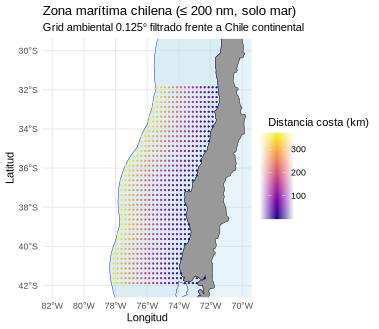
\includegraphics[width=0.8\linewidth]{figs/env_data_map} 

}

\caption{Geographical extent of the study area used for environmental covariates limited to the Chilean Exclusive Economic Zone}\label{fig:figEnvData}
\end{figure}

\subsubsection{To be requested}\label{to-be-requested}

\begin{itemize}
\tightlist
\item
  Diesel cost.
\item
  Permits by vessels
\item
  Quota prices?

  \begin{itemize}
  \tightlist
  \item
    Auction market but also secondary market if available

    \begin{itemize}
    \tightlist
    \item
      If no data, maybe intrapolate prices from other auctions?
    \end{itemize}
  \item
    Captures elements of forward-looking behavior and information
    (\citeproc{ref-Birkenbach2024}{Birkenbach et al., 2024}). Reimer et al. (\citeproc{ref-reimer2022structural}{2022}) similarly argue that
    including a quota price captures forward looking behavior and
    allows one to simplify the dynamic model to a static one.
  \end{itemize}
\item
  Quota by area/fishing organization for Artisanal, and TAC for
  industrial with ITQ (by vessel?)
\end{itemize}

\subsection{Future data for projections}\label{future-data-for-projections}

\begin{itemize}
\tightlist
\item
  OracleBio

  \begin{itemize}
  \tightlist
  \item
    Unfurtunally, only decadal (e.g., 2040--2050) projections for
    different scenarios for SST, salinity, currents and chlorophyll
    (4km resolution)
  \item
    No winds; CMIP6 for winds? (\textasciitilde100 km).
  \end{itemize}
\end{itemize}

\subsection{Econometrics models}\label{econometrics-models}

\subsubsection{Stock dynamics}\label{stock-dynamics}

To estimate stock dynamics, we use annual data on species-specific biomass (stock abundance) and vessel landings within Chile's Exclusive Economic Zone (EEZ). Following Kasperski (\citeproc{ref-Kasperski2015-jm}{2015}), the baseline model for the interannual growth of each species \(i\) is represented by a discrete logistic function that accounts for intra- and inter-species interactions:

\begin{equation}
x_{i,y+1} + h_{iy} = \underbrace{(1 + r_i)x_{iy} + \eta_i x_{iy}^2}_{R_i(x_{iy})} + \underbrace{\sum_{j \neq i}^{n-1} a_{ij} x_{iy} x_{jy}}_{I_i(x_y)} \quad i=1,\ldots,n
\label{eq1}
\end{equation}

where \(x_{iy}\) is the biomass of species \(i\) in year \(y\), \(n\) is the total number of species, \(h_{iy}\) is the annual harvest, \(r_i\) is the intrinsic growth rate, \(\eta_i\) is the density-dependent parameter, and \(\alpha_{ij}\) captures pairwise species interactions. The system of \(n\) growth equations is
estimated simultaneously using Seemingly Unrelated Regression (SUR). Following Richter et al. (\citeproc{ref-Richter2018}{2018}), we augment \eqref{eq1} by including environmental covariates \(Env_{iy}\) that affect stock dynamics, along with an error term \(\varepsilon_{iy}\) representing stochastic recruitment:

\begin{equation}
x_{i,y+1} + h_{iy} = \underbrace{(1 + r_i)x_{iy} + \eta_i x_{iy}^2}_{R_i(x_{iy})} + \underbrace{\sum_{j \neq i}^{n-1} a_{ij} x_{iy} x_{jy}}_{I_i(x_y)} + \rho_i Env_{iy} + \varepsilon_{iy} \quad i=1,\ldots,n
\label{eq2}
\end{equation}

where \(\rho_i\) denotes the environmental response parameters. Importantly, each species has its own equation, allowing for species-specific growth, density dependence, and environmental sensitivities.

Environmental conditions were summarized annually using sea surface temperature (SST) and chlorophyll-a concentration (CHL), both averaged over the South-Central Chile region within the EEZ. These variables were selected due to their recognized influence on small pelagic productivity and spatial distribution (\citeproc{ref-Axbard2016}{Axbard, 2016}). To capture nonlinear responses, we include both linear and quadratic terms for SST and CHL. Early specifications also tested wind effects, but excluding them did not reduce explanatory power (\(\text{F}_{6,21} = 0.919\), \(p\text{-value} = 0.509\)).

SST serves as a proxy for large-scale oceanographic regimes (warm vs.~cold phases) that shape recruitment success along the Humboldt Current System. Anchoveta typically dominates during cold, nutrient-rich phases, whereas sardine tends to increase under warmer regimes (\citeproc{ref-cahuin2009}{Cahuin et al., 2009}; \citeproc{ref-Yuxe1uxf1ez2014}{Yáñez et al., 2014}). CHL reflects interannual variation in primary productivity, which forms the energetic base sustaining small pelagics. As emphasized by Sumaila et al. (\citeproc{ref-sumaila2011}{2011}), ``Changes in primary productivity and planktonic community structure affect the amount of energy transferred to higher trophic levels and, eventually, the productivity of trophic groups that contribute to fisheries catches'' (see also \citeproc{ref-cheung2008}{Cheung et al., 2008}; \citeproc{ref-jennings2008}{Jennings et al., 2008}).

Figure \ref{fig:biomass} shows that anchoveta, sardine, and jack mackerel exhibit distinct biomass trajectories over time, with no evidence of strong interannual co-movement across species. Biomass levels differ markedly between them, and the figure suggests only limited interrelation alongside clear divergences in year-to-year dynamics. Harvest pressure is also visibly associated with these fluctuations; for instance, jack mackerel experienced an abrupt decline during the late 2000s, consistent with the combined effects of intense fishing pressure and unfavorable environmental conditions.

\begin{figure}[ht!]

{\centering \includegraphics{manuscript_files/figure-latex/biomass-1} 

}

\caption{Estimated biomass of small pelagic species in Chile (2000–2024)}\label{fig:biomass}
\end{figure}

The SUR framework is particularly suited to this multi-species setting, as it allows for contemporaneous correlation among residuals that naturally arise from shared environmental shocks, trophic linkages, and imperfectly observed ecological processes. Cross-species interaction terms are specified between predator (jack mackerel) and prey (anchoveta, sardine) pairs, enabling the model to capture both direct biological coupling and environmental spillovers transmitted across species. We estimate a three-equation SUR system using the SEM framework implemented in lavaan, freely allowing the error terms across biomass equations to be correlated. The model is estimated via robust maximum likelihood (MLR), yielding SUR coefficients with Huber--White robust standard errors.

\subsubsection{Trip level cost functions}\label{trip-level-cost-functions}

\begin{itemize}
\tightlist
\item
  Sumaila et al. (\citeproc{ref-sumaila2011}{2011}): ``Capital costs, that is, the cost of vessels, fishing
  gear, processing plants and so on, would be affected by climate
  change if additional capital for fishing and process ing operations
  is required to adapt to climate change impacts on the quantity,
  composition and distribution of fisheries resources65. Changes in
  migratory routes and fish distribution would affect travel time,
  which can lead to increases or decreases in fuel and ice cost
  depending on catch levels and patterns, and the management regime in
  place.''
\end{itemize}

Ignoring trip subscript, the cost functions vary by vessel
\(v=1,\ldots,V_g\) and gear used \(g=1,\ldots,G\), where \(V_g\) is the number
of observations using gear type \(g\), and \(G\) is the total number of
available (or observed) gears: \begin{equation}
C_{vg} = \sum_{i=1}^{2n+M+k} \alpha_{g, \mathbf{X}_i} \mathbf{X}_{ivg} + \frac{1}{2} \sum_{i=1}^{2n+M+k} \sum_{j=1}^{2n+M+k} \alpha_{g, \mathbf{X}_i\mathbf{X}_j} \mathbf{X}_{ivg} \mathbf{X}_{jvg}
\label{eq3}
\end{equation} where \(C_{vg}= w z_{vg}^*\),
\(\mathbf{X}_{vg}=[w;h_{vg};x;Z_v]\), \(w\) is a \(V_g \times M\) matrix of
variable input prices, \(h_{vg}\) is an \(V_g \times n\) matrix of harvest
quantities, \(x\) is an \(V_g \times n\) matrix of given stock levels of the
species of interest, and \(Z_v\) is an \(V_g \times k\) matrix of given
vessel characteristics. Therefore, \(\mathbf{X}_{vg}\) is a
\(V_g \times (2n+M+k)\) matrix, and \(\mathbf{X}_{ivg}\) represents the
\emph{i}th column of the \(\mathbf{X}_{vg}\) matrix.

Together with estimating the restricted cost function, we estimate the
conditional input demand equations. This addition allows an increase in
the degrees of freedom by imposing cross-equation parameter constraints
and allows for the testing of, for instance, jointness in inputs
(\citeproc{ref-Kasperski2015-jm}{Kasperski, 2015}). The conditional input demand equations are derived
by Shepard's Lemma: \begin{equation}
\frac{\partial C_{vg}}{\partial w_m} = z^*_{vg,w_m} = \alpha_{g,w_m} + \sum_{j=1}^{2n+M+k} \alpha_{g,w_m,\mathbf{X}_j} \mathbf{X}_{jvg} \quad m=1,\ldots,M.
\label{eq4}
\end{equation}

Similar to stock dynamics, the system of equations formed by \eqref{eq3}
and \eqref{eq4} can be estimated using SUR. To comply with economic
theory, and to reduce even more the number of parameters to estimate,
the following restrictions are imposed when estimating \eqref{eq4}:

\begin{enumerate}
\def\labelenumi{\arabic{enumi}.}
\item
  Symmetry of the cost function, where \begin{equation*}
    \alpha_{g,\mathbf{X}_i\mathbf{X}_j} = \alpha_{g,\mathbf{X}_j\mathbf{X}_i} \quad \forall \quad i=1,\ldots,(2n + M + k); \ i \neq j; \ g = 1,\ldots, G.
    \end{equation*}
\item
  Linear homogeneity in input prices, where \begin{equation*}
    \sum_m^M \alpha_{g,w_m} = 1 \ \text{and} \ \sum_m^M \alpha_{g,w_m,\mathbf{X}_i} = 0 \quad i=1,\ldots,(2n + M + k); \ g = 1,\ldots, G.
    \end{equation*}
\end{enumerate}

Data at the trip level is available upon request from the Chilean
Fisheries Research Institute (IFOP), which registers geo-referenced
catch information on the Chilean fleet's fishing operation per trip (see
e.g. \citeproc{ref-Pena-Torres2017-gn}{Peña-Torres et al., 2017} and \href{ifop.dataobservatory.net}{IFOP data
observatory}). As inputs we can use the time
spent at sea during a trip, where the price is the average wage pay to
crew member per hour, and the distance traveled during a trip, where the
price of distance traveled is the diesel cost. Therefore, the total cost
function \(C_{vg}= w z_{vg}^*\) for vessel \(v\), using gear \(g\) in a trip
would be sum of the total cost of distance travelled plus the total cost
of the time spent at sea.

\textbf{Note:} \emph{Depending on the type of vessel, this cost should change.
Some vessels are more efficient, other one are more heavy. How to
capture this? The righ hand side has vessel characteristics, so the
effect of harvest would be conditional on vessel characteristics, the
stock levels and input prices. As we only care in the margin how harvest
increase cost, this should be fine. Kasperski (\citeproc{ref-Kasperski2015-jm}{2015}) mention this
``\ldots no reliable fixed cost information on these vessels exists, but
these should not affect the optimization as economic decisions are made
at the margin. Therefore, this study does not measure true profit, but
rather a proxy based on the net operating rent accruing to vessels in
the fishery.''}

To link this function to climate change, we can also include additional
environmental variables \(Env\) to \(\mathbf{X}_{vg}\) such as wind
intensity and wave conditions in each trip at the harvest location, upon
data availability. Therefore, the augmented \(X_{vg}\) matrix becomes
\(\mathbf{X}^{'}_{vg} = [w;h_{vg};x;Z_v;Env]\).

MAYBE INCLUDE QUOTA PRICE? \textbf{Higher quota prices for depleted stocks
(e.g., GOM cod) reduce incentives to target them.} and \textbf{Active leasing
markets for quota (and previously for DAS) allow fishermen to treat
quota as a ``priced input'' rather than a fixed, exhaustible resource.}

Add - liters/hours x hours trip x fuel price - crew member x harvest x
price x share - certification cost per landed ton x landing

\subsubsection{Total annual trips}\label{total-annual-trips}

The number of trips a vessel will take in a given year for each gear
type used is assumed to follow a Poison distribution
(\citeproc{ref-Kasperski2015-jm}{Kasperski, 2015}): \begin{equation}
Pr\left[T^{*}_{vgy} = t_v\right] = \frac{exp^{-exp(U^{'}_{vg}\beta_g)}exp(U^{'}_{vg}\beta_g)^{t_v}}{t_v !}
\label{eq5}
\end{equation} where \(U_{vg}=[p,w,h_{vg},\bar{q},Z_{vg}]\) is a
\((3n+M+k+1)×V_g\) matrix of explanatory variables, \(\beta_g\) is a
\((3n+M+k+1)\times1\) matrix of coefficients to be estimated, \(t_v\) is the
number of trips taken by vessel \(v\) using gear type \(g\) in year \(y\), and
\(\bar{q}\) is the annual quota level. Additionally, we can add the
accumulation of ``bad weather days'' as an explanatory variable to
incorporate weather conditions into this decision, thus
\(U_{vg}=[p,w,h_{vg},\bar{q},Z_{vg}, Env]\)

De Dresdner 2014: - Regulacion: Numero de dias de vedas / Cuota anual -
Precios: Precio proceso + Precio Diesel (promedio meses de mayor
productividad en la pesquería (marzo a junio y octubre a diciembre). -
Agregar Precio quota?

\subsubsection{Inverse demand model}\label{inverse-demand-model}

The price of each species is modeled using an Inverse Almost Ideal
Demand System (IADS). The price of a species \(i\) in year \(y\) is the
following:

\begin{equation}
\ln p_{iy} = \sum_j^n \gamma_j \ln h_{j,y} + \gamma_{H} \ln H + \gamma_{FM} \ln P^\text{FishMeal} + \epsilon_{iy}, \quad i = 1,\ldots,n, \ j = 1,\ldots,n.
\label{eq6}
\end{equation}

Note that harvest may be endogenous in this system due to simultaneity.
For this reason, the system formed by \eqref{eq6} will be estimated
using a Three Stage Least Squares (3SLS) procedure, where h\_j\{j,y\} would
be instrumented by variables that affect the fishers' supply function
such as SST, Chl, and fuel prices.

\begin{itemize}
\tightlist
\item
  DIFERENCIAR ENTRE CONSUMO HUMANO DIRECTO e INDIRECTO? Ricardo y Arnol usan solo información de procesamiento. Darle una vuelta a esto
\end{itemize}

\subsection{Numerical optimization}\label{numerical-optimization}

To obtain the effect of future climate variability on stock, harvest,
quota and profits, we conduct numerical optimization for different
climate scenarios using the parameters estimates for the stock dynamic,
cost functions, total annual trips and inverse demand equations. In each
year, a vessel maximizes profits by choosing their optimal number of
trips \(T_g\) and harvest levels per trip \(h_{g\tau}\) given a gear type:
\begin{align}
\max_{h_{gt}, T_g} \quad \pi_{vgt} & = \sum_{\tau=t}^{T_g} \rho^\tau \left\{ P(h) h_{g\tau} - C_g(h_{g\tau} | w, x, Z, Env) \right\} \quad \tau = t,\ldots, T_g \nonumber \\
\textbf{s.t} \quad q_{g,t+1} & = \omega \ast \bar{q} - \sum_{t=1}^{t} h_{gt} \geq 0, \quad t = 1, \dots, T-1, \quad g = 1, \dots, G
\label{eq7}
\end{align} where \(\rho\) is the intra-annual discount factor, \(\omega\)
is a vector of shares of \(\bar{q}\), and \(h_{lt}=0\) for all \(l\neq g\).
The vector of shares is obtained from historical data on harvest. The
optimal profit from the maximization problem in \eqref{eq7} is denoted
as \(\pi_{vgy}^* (p,w,x,Z,\bar{q},\omega, Env)\), and \(h_{vgty}^*\) and
\(T_{vgy}^*\) are the optimal choices harvest per trip and total number of
trips in year \(y\) for vessel \(v\). To obtain the optimal quota level, we
must solve the social-planner optimization problem to maximize the net
value of the fishery by choosing the quota levels per year and by
species.

Following Kasperski (\citeproc{ref-Kasperski2015-jm}{2015}), the optimization problem will be conducted
for the next 25 years. I will use different climate scenarios and
compare different optimal outcomes between them by using future
projections for the environmental variables included in the model.

\begin{itemize}
\tightlist
\item
  Note that the optimal quota would that we would find using
  historical data might differ from the actual quota set by the
  regulator as they model is for single species.
\end{itemize}

\subsection{Projections}\label{projections}

\emph{From (\citeproc{ref-Yuxe1uxf1ez2014}{Yáñez et al., 2014})}:

\begin{itemize}
\tightlist
\item
  ``To project the model, the average structure of catches and
  temperature (of Antofagasta and the region Niño 3 + 4) for the years
  2005, 2006 and 2007 were used as starting point. We consider a
  linear increase in temperature, taking into account four climate
  change scenarios based on the scenarios presented by IPCC, designed
  for the northern part of Chile until 2100.

  \begin{enumerate}
  \def\labelenumi{\arabic{enumi}.}
  \tightlist
  \item
    The first scenario considers an increase in temperature of
    0.034ºC per year (\citeproc{ref-Fuenzalida2007}{Fuenzalida et al., 2007}), similar to that estimated by

    \begin{enumerate}
    \def\labelenumii{\arabic{enumii}.}
    \tightlist
    \item
    \end{enumerate}
  \item
    A second scenario, more moderate, of 0,025ºC/year is also
    proposed by Fuenzalida et al. (\citeproc{ref-Fuenzalida2007}{2007}).
  \item
    The third scenario is not considered a significant effect on the
    area, following the work of 1.
  \item
    The fourth scenario is contradictory, indicating a cooling de
    0.02 ºC/year (\citeproc{ref-falvey2009}{Falvey \& Garreaud, 2009}). It should be noted that according to
    the work of Fuenzalida et al. (\citeproc{ref-Fuenzalida2007}{2007}) and Falvey \& Garreaud (\citeproc{ref-falvey2009}{2009}) the same SST
    increase (or decrease) were considered for both temperatures (in
    Antofagasta and in the Niño 3 + 4 region).''
  \end{enumerate}
\end{itemize}

\section{Results}\label{results}

\subsection{Stock biomass model}\label{stock-biomass-model}

PROBAR CON SOLO INTERACCION CON MACKEREL!!! (Pray and predator model)

Figure \ref{fig:harvestbiomass} show biomass adding harvest

\begin{figure}[ht!]

{\centering \includegraphics{manuscript_files/figure-latex/harvestbiomass-1} 

}

\caption{Estimated biomass vs harvest of small pelagic species in CentralSouth Chile (2000–2024)}\label{fig:harvestbiomass}
\end{figure}

Estimar modelo

Table \ref{tab:SUR_results} reports the SUR estimates of annual biomass dynamics for sardine, anchoveta, and jack mackerel using robust standard errors. Including sea surface temperature (SST) and chlorophyll-a (CHL) significantly improves model performance, leading us to reject the joint exclusion of environmental covariates at the 10\% significance level (F\(_{12,27}\) = 1.874, \(p\)-value = 0.07).

The three species exhibit strong interannual persistence and significant density dependence, consistent with discrete logistic growth. Sardine biomass responds positively to chlorophyll-a concentration and negatively to SST, indicating that productivity-rich and cooler conditions enhance its growth. This SST response contrasts with evidence from the California Current, where sardine abundance tends to increase under warm regimes (\citeproc{ref-Herrick2009}{Herrick et al., 2009}). \textbf{IS THIS TRUE FOR CHILE?} Anchoveta shows a similar negative response to temperature, together with pronounced density dependence, reflecting its high environmental sensitivity. In contrast, jack mackerel displays weaker environmental dependence, but its SST quadratic term is significant, suggesting a thermal optimum and reduced biomass under extreme temperatures.

Cross-species effects reveal one notable ecological interaction: anchoveta biomass declines in years with high sardine biomass. \textbf{IS THIS PATTERN CONSISTEN WITH LITERATURE?}. No significant interaction effects are detected for jack mackerel, consistent with its broader spatial range and weaker coupling to coastal pelagic dynamics.

Overall, the model captures distinct species‐specific responses to environmental variability. Sardine biomass is strongly driven by ocean productivity, anchoveta by density dependence and thermal conditions, and jack mackerel by a combination of persistence and nonlinear temperature responses.

\begin{table}[!htbp]
\centering
\caption{Seemingly Unrelated Regression (SUR) estimates of biomass dynamics}
\label{tab:SUR_results}

\begingroup 
\footnotesize 
\begin{tabular}{@{\extracolsep{5pt}}lccc} 
\\[-1.8ex]\hline 
\hline \\[-1.8ex] 
 & Sardine & Anchovy & Jack mackerel \\ 
\\[-1.8ex] & (1) & (2) & (3)\\ 
\hline \\[-1.8ex] 
 Sardine biomass (t) & 0.366$^{**}$ (0.152) &  &  \\ 
  Sardine biomass (t)$^2$ & $-$0.008 (0.011) &  &  \\ 
  Anchovy biomass (t) &  & 1.212$^{***}$ (0.205) &  \\ 
  Anchovy biomass (t)$^2$ &  & $-$0.233$^{***}$ (0.041) &  \\ 
  Jack mackerel biomass (t) &  &  & 0.903$^{***}$ (0.140) \\ 
  Jack mackerel biomass (t)$^2$ &  &  & $-$0.023$^{***}$ (0.006) \\ 
  SST & $-$20.122$^{***}$ (4.171) & $-$6.062$^{***}$ (2.162) & 13.033$^{**}$ (5.801) \\ 
  SST$^2$ & 42.107$^{*}$ (22.300) & $-$8.483 (9.298) & $-$49.589$^{**}$ (23.583) \\ 
  Chlorophyll-a & 87.856$^{***}$ (19.053) & 1.030 (14.722) & 6.583 (32.068) \\ 
  Chlorophyll-a$^2$ & $-$240.056 (200.636) & $-$115.129 (171.700) & 380.375 (295.463) \\ 
  Sardine × Anchovy & $-$0.010 (0.027) & $-$0.028$^{**}$ (0.012) &  \\ 
  Sardine × Jack mackerel & 0.008 (0.010) &  & $-$0.006 (0.008) \\ 
  Anchovy × Jack mackerel &  & $-$0.009 (0.020) & 0.030 (0.033) \\ 
  Constant & 25.350$^{***}$ (4.090) & 13.079$^{***}$ (2.515) & 28.717$^{***}$ (5.613) \\ 
 \hline \\[-1.8ex] 
Observations & 18 & 18 & 18 \\ 
R$^{2}$ & 0.772 & 0.621 & 0.858 \\ 
Adjusted R$^{2}$ & 0.570 & 0.285 & 0.731 \\ 
Residual Std. Error (df = 9) & 8.329 & 4.774 & 10.543 \\ 
\hline 
\hline \\[-1.8ex] 
\textit{Note:}  & \multicolumn{3}{r}{*$p<0.1$; **$p<0.05$; ***$p<0.01$. Robust standard errors in parenthesis.} \\ 
\end{tabular} 
\endgroup 
\end{table}

\subsection{Trip level costo function}\label{trip-level-costo-function}

EMPEZAR A ESTIMAR ESTO!!!! USANDO LOGBOOKS

\textless\textless{} NO RESULTS YET \textgreater\textgreater{}

\subsection{Total Annual trips}\label{total-annual-trips-1}

\textless\textless{} NO RESULTS YET \textgreater\textgreater{}

\subsection{Inverse demand model}\label{inverse-demand-model-1}

\textless\textless{} NO RESULTS YET \textgreater\textgreater{}

Two undergrad students working on this module for their thesis\ldots{}
Results by July 2026

\subsection{Numerical optimization}\label{numerical-optimization-1}

\textless\textless{} NO RESULTS YET \textgreater\textgreater{}

Once I have results for the four models, then I can run optimizations

\section{Discussion}\label{discussion}

\begin{itemize}
\tightlist
\item
  From Sumaila et al. (\citeproc{ref-sumaila2011}{2011}): ``A shift in species' geographic range will thus
  affect the distribution and composition of fisheries resources. This
  may affect fishing operations, the allocation of catch shares and
  the effectiveness of fisheries management measures''
\item
  For the ITQ fisheries (i.e., industrial jack mackerel?:

  \begin{itemize}
  \tightlist
  \item
    The theoretical findings on multispecies harvest patterns in
    Birkenbach et al. (\citeproc{ref-Birkenbach2020-nh}{2020}) give rise to nuanced hypotheses about how
    behavior and outcomes will change after the adoption of catch
    shares. For example, a secure property right to catch fish at
    any time in the fishing season allows firms to spread the catch
    of stocks with high prices and downward-sloping demand over a
    longer fishing season. This minimizes market gluts that steer
    product toward lower priced frozen markets (\citeproc{ref-homans2005}{Homans \& Wilen, 2005}) and can
    result in higher prices for those species. Fishermen might also
    shift their efforts toward lower-priced species with cheaper
    quota or toward non-catch-share fisheries, intensifying the race
    to fish for those species during portions of the season
    (\citeproc{ref-asche2007}{Asche et al., 2007}; \citeproc{ref-cunningham2016spillovers}{Cunningham et al., 2016}).

    \begin{itemize}
    \tightlist
    \item
      However, we do not include other species than jack mackerel,
      sardine and anchovy that might be caught by thise fleet.
      This would require too expand the model by \textbf{N} species,
      which would increase dimensionality of the model.
    \item
      We need permits to check if actually this happen (\ldots{} still
      problem with Open-Access fisheries that do not require
      permits)
    \end{itemize}
  \end{itemize}
\item
  Although the present model captures the historical relationships
  between biomass, temperature, and productivity, future strengthening
  of coastal winds and warming of the Chilean coast (Fuenzalida et al.
  2007; Garreaud et al.~2009) could shift these dynamics, altering
  species overlap and fishery composition.
\item
  About using CHL for future predictions.

  \begin{itemize}
  \tightlist
  \item
    From Sumaila et al. (\citeproc{ref-sumaila2011}{2011}): ``However, our understanding of the magnitude
    and direction of climate change effects on primary productivity
    is uncertain. For example, projections of primary production
    based on an empirical relationship estimate increases of
    0.7--8.1\% by 2050 relative to 2000 (ref. 39), whereas outputs
    from four Earth-system models suggest a possible decrease of
    2--20\% by 2100 relative to pre-industrial conditions12. The
    opposite trends and the large regional differences of the
    estimates highlight the uncertainty in the projection of
    large-scale changes in primary productivity''.
  \end{itemize}
\item
  About prices (\citeproc{ref-sumaila2011}{Sumaila et al., 2011}):

  \begin{itemize}
  \tightlist
  \item
    ``Everything being equal, when climate change reduces fish
    supply, fish price should increase, which could be large enough
    to balance out the loss in gross revenues due to reduced
    catches. However, consumers may seek substitutes as prices
    increase, thereby dampening the demand for fish and reducing the
    potential for price increases.''
  \item
    ``Ex-vessel revenues can be affected by climate change through
    effects first on the quantity, quality and distribution of
    catches, and then, on ex-vessel prices of fish.''
  \end{itemize}
\item
  Adaptation (\citeproc{ref-sumaila2011}{Sumaila et al., 2011}):

  \begin{itemize}
  \tightlist
  \item
    ``When climate change affects the composition and productivity of
    exploited species in a region, some fishers can adapt by
    switching target species or gear type81 or by moving to
    marginally productive areas. Grafton, R. Q. Adaptation to
    climate change in marine capture fisheries. Mar.~Policy 34,
    606--615 (2010).''

    \begin{itemize}
    \tightlist
    \item
      ``For example, new fisheries have already developed for
      several southern species in the UK (for example, red mullet)
      as these species have started to migrate to the North Sea
      because of an increase in sea temperature. Beare, D. J. et
      al.~Long-term increase in prevalence of North Sea fishes
      having southern biogeographic affinities. Mar.~Ecol. Prog.
      Ser. 284, 269--278 (2004).''
    \item
      ``The ability of fishers and fishing enterprises to adapt
      depends on a number of factors, including the mobility of
      the fishing fleet. -''At present, the dominant hypothesis is
      that more technologically advanced fleets, usually located
      in rich northern countries, are more likely to be better
      prepared to adapt to climate change by moving to other
      fishing grounds and by shifting gears. MacNeil, M. A. et al.
      Transitional states in marine fisheries: adapting to
      predicted global change. Phil. Trans. R. Soc. B 365,
      3753--3763 (2011).''
    \end{itemize}
  \end{itemize}
\item
  we did not added production risk\ldots. risk preferences? maybe using
  random coefficients? Discusse!!!
\end{itemize}

\section{Conclusions}\label{conclusions}

NO YET!

\subsection{Future research question}\label{future-research-question}

\begin{itemize}
\item
  Several other extensions to the model can be incorporated to be
  improved. For instance, the geographical space where fishermen
  operate is relevant, as depending on the location chosen and when to
  participate, the set of potential choices would vary
  (\citeproc{ref-Reimer2017-jw}{Reimer et al., 2017}). As I mentioned above, it is possible to extend the
  stock dynamic model by considering different locations. The model
  would also require that the participation decision, which is
  captured by the Poisson model on the annual number of trips, should
  then consider the decision to participate in a determined fishing
  ground, connecting the multispecies model of Kasperski (\citeproc{ref-Kasperski2015-jm}{2015}) to
  the literature of location choice modeling (e.g., \citeproc{ref-Dupont1993-jn}{Dupont, 1993}; \citeproc{ref-Hicks2020-mz}{Hicks et al., 2020}; \citeproc{ref-Smith2005-us}{Smith, 2005}).

  \begin{itemize}
  \tightlist
  \item
    About the DCM?

    \begin{itemize}
    \tightlist
    \item
      Including other economic activity would be relevant, as
      aquaculture is become more relevant in the country, where
      some fishermen have swith to small-scale aquaculture
      practice.
    \item
      Outside option\ldots{}
    \end{itemize}
  \end{itemize}
\item
  Does higher quota allocation of jack mackerel, a predator for
  anchovy and sardine, helps small scale sector actually?
\end{itemize}

\section{Repository}\label{repository}

The source code for this project is available on
\href{https://github.com/fquezadae/Impact-of-Environmental-Variability-on-Harvest}{GitHub}

\section*{References}\label{references}
\addcontentsline{toc}{section}{References}

\phantomsection\label{refs}
\begin{CSLReferences}{1}{0}
\bibitem[\citeproctext]{ref-Abbott2023-sb}
Abbott, J. K., Sakai, Y., \& Holland, D. S. (2023). Species, space and time: A quarter century of fishers' diversification strategies on the {US} west coast. \emph{Fish Fish (Oxf.)}, \emph{24}(1), 93--110.

\bibitem[\citeproctext]{ref-Aguilera2015-wo}
Aguilera, S. E., Cole, J., Finkbeiner, E. M., Le Cornu, E., Ban, N. C., Carr, M. H., Cinner, J. E., Crowder, L. B., Gelcich, S., Hicks, C. C., Kittinger, J. N., Martone, R., Malone, D., Pomeroy, C., Starr, R. M., Seram, S., Zuercher, R., \& Broad, K. (2015). Managing small-scale commercial fisheries for adaptive capacity: Insights from dynamic social-ecological drivers of change in monterey bay. \emph{PLoS One}, \emph{10}(3), e0118992.

\bibitem[\citeproctext]{ref-Alheit2004}
Alheit, J., \& Niquen, M. (2004). Regime shifts in the humboldt current ecosystem. \emph{Progress in Oceanography}, \emph{60}(2-4), 201--222. \url{https://doi.org/10.1016/j.pocean.2004.02.006}

\bibitem[\citeproctext]{ref-Arancibia2019-FIPA}
Arancibia, H., Klarian, S., Alarcón, R., Barros, M., Harrod, C., Jackson, A., Schultz, E. T., Medina, M., Neira, S., \& Valdés, J. (2019). \emph{Informe final proyecto FIPA 2017-63: Conducta trófica del jurel}. Universidad de Concepción; Universidad Andrés Bello; Universidad Arturo Prat; Universidad de Antofagasta. \url{https://www.subpesca.cl/fipa/613/articles-98303_informe_final.pdf}

\bibitem[\citeproctext]{ref-asche2007}
Asche, F., Gordon, D. V., \& Jensen, C. L. (2007). Individual vessel quotas and increased fishing pressure on unregulated species. \emph{Land Economics}, \emph{83}(1), 41--49.

\bibitem[\citeproctext]{ref-Axbard2016}
Axbard, S. (2016). Income opportunities and sea piracy in indonesia: Evidence from satellite data. \emph{American Economic Journal: Applied Economics}, \emph{8}(2), 154--194. \url{https://doi.org/10.1257/app.20140404}

\bibitem[\citeproctext]{ref-Beaudreau2019-xg}
Beaudreau, A. H., Ward, E. J., Brenner, R. E., Shelton, A. O., Watson, J. T., Womack, J. C., Anderson, S. C., Haynie, A. C., Marshall, K. N., \& Williams, B. C. (2019). Thirty years of change and the future of alaskan fisheries: Shifts in fishing participation and diversification in response to environmental, regulatory and economic pressures. \emph{Fish Fish}, \emph{20}(faf.12364), 601--619.

\bibitem[\citeproctext]{ref-Birkenbach2020-nh}
Birkenbach, A. M., Cojocaru, A. L., Asche, F., Guttormsen, A. G., \& Smith, M. D. (2020). Seasonal harvest patterns in multispecies fisheries. \emph{Environ. Resour. Econ.}, \emph{75}(3), 631--655.

\bibitem[\citeproctext]{ref-Birkenbach2024}
Birkenbach, A. M., Lee, M.-Y., \& Smith, M. D. (2024). Counterfactual modeling of multispecies fisheries outcomes under market-based regulation. \emph{Journal of the Association of Environmental and Resource Economists}, \emph{11}(3), 755--796. \url{https://doi.org/10.1086/727356}

\bibitem[\citeproctext]{ref-cahuin2009}
Cahuin, S. M., Cubillos, L. A., Niquen, M., \& Escribano, R. (2009). Climatic regimes and the recruitment rate of anchoveta, engraulis ringens, off peru. \emph{Estuarine, Coastal and Shelf Science}, \emph{84}(4), 591--597.

\bibitem[\citeproctext]{ref-Carter2018}
Carter, C., Cui, X., Ghanem, D., \& Mérel, P. (2018). Identifying the economic impacts of climate change on agriculture {[}Journal Article{]}. \emph{Annual Review of Resource Economics}, \emph{10}(Volume 10, 2018), 361--380. https://doi.org/\url{https://doi.org/10.1146/annurev-resource-100517-022938}

\bibitem[\citeproctext]{ref-Cherdchuchai2006}
Cherdchuchai, S., \& Otsuka, K. (2006). Rural income dynamics and poverty reduction in thai villages from 1987 to 2004. \emph{Agricultural Economics}, \emph{35}(s3), 409--423. https://doi.org/\url{https://doi.org/10.1111/j.1574-0862.2006.00187.x}

\bibitem[\citeproctext]{ref-cheung2008}
Cheung, W. W., Close, C., Lam, V., Watson, R., \& Pauly, D. (2008). Application of macroecological theory to predict effects of climate change on global fisheries potential. \emph{Marine Ecology Progress Series}, \emph{365}, 187--197.

\bibitem[\citeproctext]{ref-Cheung2010}
Cheung, W. W., Lam, V. W., Sarmiento, J. L., Kearney, K., Watson, R., Zeller, D., \& Pauly, D. (2010). Large-scale redistribution of maximum fisheries catch potential in the global ocean under climate change. \emph{Global Change Biology}, \emph{16}(1), 24--35.

\bibitem[\citeproctext]{ref-Cline2017-dp}
Cline, T. J., Schindler, D. E., \& Hilborn, R. (2017). Fisheries portfolio diversification and turnover buffer alaskan fishing communities from abrupt resource and market changes. \emph{Nat. Commun.}, \emph{8}, 14042.

\bibitem[\citeproctext]{ref-sjcruz_jmp}
Cruz, S. J. (2025). \emph{Climate variability and labor allocation: Evidence from mexican small-scale fisheries}. Working Paper. \url{https://sjcruz.github.io/publication/jmp/}

\bibitem[\citeproctext]{ref-cunningham2016spillovers}
Cunningham, S., Bennear, L. S., \& Smith, M. D. (2016). Spillovers in regional fisheries management: Do catch shares cause leakage? \emph{Land Economics}, \emph{92}(2), 344--362.

\bibitem[\citeproctext]{ref-Dupont1993-jn}
Dupont, D. P. (1993). Price uncertainty, expectations formation and fishers' location choices. \emph{Mar. Resour. Econ.}, \emph{8}(3), 219--247.

\bibitem[\citeproctext]{ref-Ellis2000}
Ellis, F. (2000). The determinants of rural livelihood diversification in developing countries. \emph{Journal of Agricultural Economics}, \emph{51}(2), 289--302. https://doi.org/\url{https://doi.org/10.1111/j.1477-9552.2000.tb01229.x}

\bibitem[\citeproctext]{ref-GlobColour}
E.U. Copernicus Marine Service Information. (2025a). \emph{Global ocean colour (copernicus-GlobColour)}. Marine Data Store (MDS). \url{https://doi.org/10.48670/moi-00281}

\bibitem[\citeproctext]{ref-WIND_GLO_PHY}
E.U. Copernicus Marine Service Information. (2025b). \emph{Global ocean hourly reprocessed sea surface wind and stress from scatterometer and model}. Marine Data Store (MDS). \url{https://doi.org/10.48670/moi-00185}

\bibitem[\citeproctext]{ref-GLORYS12V1}
E.U. Copernicus Marine Service Information. (2025c). \emph{Global ocean physics reanalysis}. Marine Data Store (MDS). \url{https://doi.org/10.48670/moi-00021}

\bibitem[\citeproctext]{ref-falvey2009}
Falvey, M., \& Garreaud, R. D. (2009). Regional cooling in a warming world: Recent temperature trends in the southeast pacific and along the west coast of subtropical south america (1979--2006). \emph{Journal of Geophysical Research: Atmospheres}, \emph{114}(D4).

\bibitem[\citeproctext]{ref-Finkbeiner2015-bs}
Finkbeiner, E. M. (2015). The role of diversification in dynamic small-scale fisheries: Lessons from baja california sur, mexico. \emph{Glob. Environ. Change}, \emph{32}, 139--152.

\bibitem[\citeproctext]{ref-Fisher2021-lw}
Fisher, M. C., Moore, S. K., Jardine, S. L., Watson, J. R., \& Samhouri, J. F. (2021). Climate shock effects and mediation in fisheries. \emph{Proc. Natl. Acad. Sci. U. S. A.}, \emph{118}(2).

\bibitem[\citeproctext]{ref-Frawley2021-cw}
Frawley, T. H., Muhling, B. A., Brodie, S., Fisher, M. C., Tommasi, D., Le Fol, G., Hazen, E. L., Stohs, S. S., Finkbeiner, E. M., \& Jacox, M. G. (2021). Changes to the structure and function of an albacore fishery reveal shifting social‐ecological realities for pacific northwest fishermen. \emph{Fish Fish}, \emph{22}(2), 280--297.

\bibitem[\citeproctext]{ref-Free2019}
Free, C. M., Thorson, J. T., Pinsky, M. L., Oken, K. L., Wiedenmann, J., \& Jensen, O. P. (2019). Impacts of historical warming on marine fisheries production. \emph{Science}, \emph{363}(6430), 979--983. \url{https://doi.org/10.1126/science.aau1758}

\bibitem[\citeproctext]{ref-Fuenzalida2007}
Fuenzalida, H., Aceituno, P., Falvey, M., Garreaud, R., Rojas, M., \& Sánchez, R. (2007). \emph{Study on climate variability for chile during the 21st century} {[}Technical report{]}. National Environmental Committee.

\bibitem[\citeproctext]{ref-Gonzalez-Mon2021-kj}
Gonzalez-Mon, B., Bodin, Ö., Lindkvist, E., Frawley, T. H., Giron-Nava, A., Basurto, X., Nenadovic, M., \& Schlüter, M. (2021). Spatial diversification as a mechanism to adapt to environmental changes in small-scale fisheries. \emph{Environ. Sci. Policy}, \emph{116}, 246--257.

\bibitem[\citeproctext]{ref-Herrick2009}
Herrick, S. F. Jr. et al. (2009). Lobal production and economics. In D. M. Checkley, C. Roy, J. Alheit, \& Y. Oozeki (Eds.), \emph{Climate change and small pelagic fish} (pp. 256--274). Cambridge University Press.

\bibitem[\citeproctext]{ref-Hicks2020-mz}
Hicks, R. L., Holland, D. S., Kuriyama, P. T., \& Schnier, K. E. (2020). Choice sets for spatial discrete choice models in data rich environments. \emph{Res. Energy Econ.}, \emph{60}, 101148.

\bibitem[\citeproctext]{ref-homans2005}
Homans, F. R., \& Wilen, J. E. (2005). Markets and rent dissipation in regulated open access fisheries. \emph{Journal of Environmental Economics and Management}, \emph{49}(2), 381--404.

\bibitem[\citeproctext]{ref-Jardine2020-um}
Jardine, S. L., Fisher, M. C., Moore, S. K., \& Samhouri, J. F. (2020). Inequality in the economic impacts from climate shocks in fisheries: The case of harmful algal blooms. \emph{Ecol. Econ.}, \emph{176}, 106691.

\bibitem[\citeproctext]{ref-jennings2008}
Jennings, S., Mélin, F., Blanchard, J. L., Forster, R. M., Dulvy, N. K., \& Wilson, R. W. (2008). Global-scale predictions of community and ecosystem properties from simple ecological theory. \emph{Proceedings of the Royal Society B: Biological Sciences}, \emph{275}(1641), 1375--1383.

\bibitem[\citeproctext]{ref-Kasperski2015-jm}
Kasperski, S. (2015). Optimal multi-species harvesting in ecologically and economically interdependent fisheries. \emph{Environ. Resour. Econ.}, \emph{61}(4), 517--557.

\bibitem[\citeproctext]{ref-Kasperski2013-jz}
Kasperski, S., \& Holland, D. S. (2013). Income diversification and risk for fishermen. \emph{Proc. Natl. Acad. Sci. U. S. A.}, \emph{110}(6), 2076--2081.

\bibitem[\citeproctext]{ref-Pena-Torres2017-gn}
Peña-Torres, J., Dresdner, J., \& Vasquez, F. (2017). El niño and fishing location decisions: The chilean straddling jack mackerel fishery. \emph{Mar. Resour. Econ.}, \emph{32}(3), 249--275.

\bibitem[\citeproctext]{ref-peuxf1a_torres_2022_MRE}
Peña-Torres, J., Muñoz, R., Quezada, F., \& Kaufmann, C. (2022). Entry deterrence and collusion at repeated multiunit auctions of ITQs. \emph{Marine Resource Economics}, \emph{37}(4), 437--465. \url{https://doi.org/10.1086/721014}

\bibitem[\citeproctext]{ref-Poloczanska2013-qq}
Poloczanska, E. S., Brown, C. J., Sydeman, W. J., Kiessling, W., Schoeman, D. S., Moore, P. J., Brander, K., Bruno, J. F., Buckley, L. B., Burrows, M. T., Duarte, C. M., Halpern, B. S., Holding, J., Kappel, C. V., O'Connor, M. I., Pandolfi, J. M., Parmesan, C., Schwing, F., Thompson, S. A., \& Richardson, A. J. (2013). Global imprint of climate change on marine life. \emph{Nat. Clim. Chang.}, \emph{3}(10), 919--925.

\bibitem[\citeproctext]{ref-Powell2022-wj}
Powell, F., Levine, A., \& Ordonez-Gauger, L. (2022). Climate adaptation in the market squid fishery: Fishermen responses to past variability associated with el niño southern oscillation cycles inform our understanding of adaptive capacity in the face of future climate change. \emph{Clim. Change}, \emph{173}(1-2), 1.

\bibitem[\citeproctext]{ref-reimer2022structural}
Reimer, M. N., Abbott, J. K., \& Haynie, A. C. (2022). Structural behavioral models for rights-based fisheries. \emph{Resource and Energy Economics}, \emph{68}, 101294.

\bibitem[\citeproctext]{ref-Reimer2017-jw}
Reimer, M. N., Abbott, J. K., \& Wilen, J. E. (2017). Fisheries production: Management institutions, spatial choice, and the quest for policy invariance. \emph{Mar. Resour. Econ.}, \emph{32}(2), 143--168.

\bibitem[\citeproctext]{ref-Richter2018}
Richter, A., Eikeset, A. M., Van Soest, D., Diekert, F. K., \& Stenseth, N. C. (2018). Optimal management under institutional constraints: Determining a total allowable catch for different northeast arctic cod fishery fleet segments. \emph{Environmental and Resource Economics}, \emph{69}, 811--835. \url{https://doi.org/10.1007/s10640-016-0106-3}

\bibitem[\citeproctext]{ref-Sethi2014-bn}
Sethi, S. A., Reimer, M., \& Knapp, G. (2014). Alaskan fishing community revenues and the stabilizing role of fishing portfolios. \emph{Mar. Policy}, \emph{48}, 134--141.

\bibitem[\citeproctext]{ref-Smith2005-us}
Smith, M. D. (2005). State dependence and heterogeneity in fishing location choice. \emph{J. Environ. Econ. Manage.}, \emph{50}(2), 319--340.

\bibitem[\citeproctext]{ref-Stafford2018-pq}
Stafford, T. M. (2018). Accounting for outside options in discrete choice models: An application to commercial fishing effort. \emph{J. Environ. Econ. Manage.}, \emph{88}, 159--179.

\bibitem[\citeproctext]{ref-SUBPESCA2020}
SUBPESCA. (2020). \emph{Informe sectorial de pesca y acuicultura 2019}. Subsecretaría de Pesca y Acuicultura. \url{https://www.subpesca.cl/portal/618/articles-106845_documento.pdf}

\bibitem[\citeproctext]{ref-sumaila2011}
Sumaila, U. R., Cheung, W. W., Lam, V. W., Pauly, D., \& Herrick, S. (2011). Climate change impacts on the biophysics and economics of world fisheries. \emph{Nature Climate Change}, \emph{1}(9), 449--456.

\bibitem[\citeproctext]{ref-Vasquez_Caballero2023-ip}
Vasquez Caballero, S., Sylvia, G., \& Holland, D. S. (2023). Fishery participation and location choice model: The west coast salmon troll commercial fishery. \emph{Can. J. Fish. Aquat. Sci.}

\bibitem[\citeproctext]{ref-Yuxe1uxf1ez2014}
Yáñez, E., Barbieri, M. A., Plaza, F., \& Silva, C. (2014). Climate change and fisheries in chile. In M. Behnassi, M. Syomiti Muteng'e, G. Ramachandran, \& K. N. Shelat (Eds.), \emph{Vulnerability of agriculture, water and fisheries to climate change: Toward sustainable adaptation strategies} (pp. 259--270). Springer Netherlands. \url{https://doi.org/10.1007/978-94-017-8962-2_16}

\bibitem[\citeproctext]{ref-Young2018-kk}
Young, T., Fuller, E. C., Provost, M. M., Coleman, K. E., St. Martin, K., McCay, B. J., \& Pinsky, M. L. (2018). Adaptation strategies of coastal fishing communities as species shift poleward. \emph{ICES Journal of Marine Science}, \emph{76}(1), 93--103.

\bibitem[\citeproctext]{ref-Zhang2011-wv}
Zhang, J., \& Smith, M. D. (2011). Heterogeneous response to marine reserve formation: {A} sorting model approach. \emph{Environ. Resour. Econ.}, \emph{49}(3), 311--325.

\end{CSLReferences}

\end{document}
